\section{Inventory}
\label{sec:inventory}

\begin{figure}[ht]
	\centering
  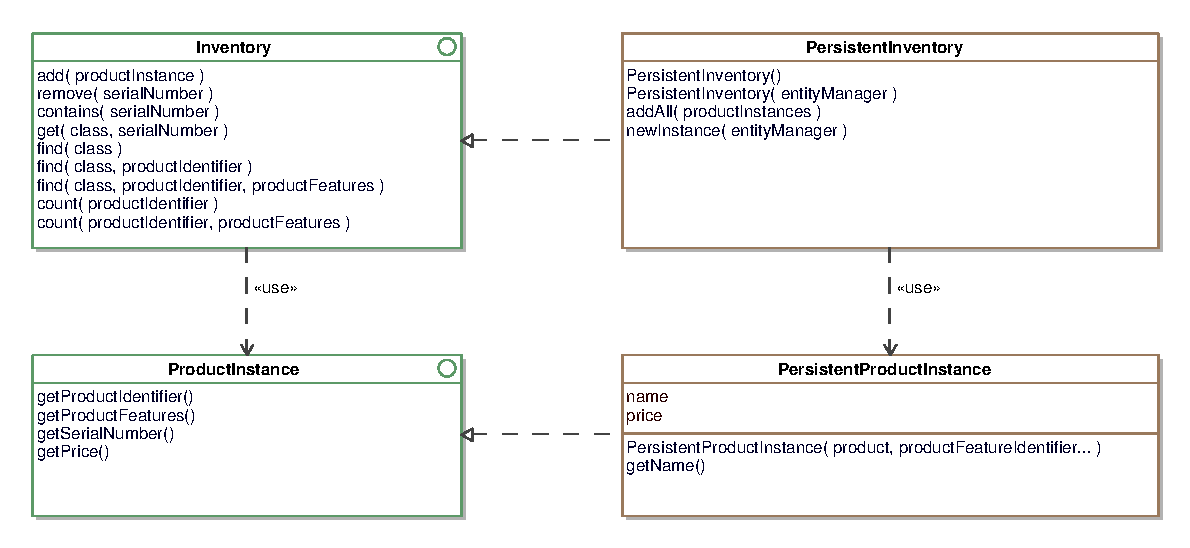
\includegraphics[width=1.0\textwidth]{images/Inventory_Overview.eps}
	\label{inventory_overview}
	\caption{Inventory - Class Overview}
\end{figure}

An inventory is a place, where products are stored.
In \salespoint{}, an abstract representation if the \code{Inventory} interface and its implementing class \code{PersistentInventory}.
The interface and declares methods to add, remove and find products.
Because an inventory contains specific product instances, \code{PersistentInventory} aggregates \code{PersistentProductInstance}s.

\code{PersistentProductInstance}s can be retrieved from \code{PersistentInventory} by specifying a \code{SerialNumber} or a \code{ProductIdentifier}.
A \code{SerialNumber} is used to reference a specific \code{ProductInstance}.
A \code{ProductIdentifier} identifies a \code{Product} uniquely, thus all \code{PersistentProductInstance}s of the \code{PersistentProduct} specified by the supplied \code{ProductIdentifier} are returned.
Additionally an \code{Iterable<ProductFeature>} can be supplied to the \code{find()}-method along with a \code{ProductIdentifier} to retrieve all instances of a product, where the \code{ProductFeature}s match exactly those specified.
Matching a set of \code{ProductFeatures} against a \code{PersistentProductInstance} is hard to express in JPQL or Criteria Queries (see Section \ref{sec:jpa}).
Therefore, only the \code{ProductIdentifier} is used to build a Criteria Query, which is executed on the database.
Selecting only those \code{PersistentProductInstances} which match the specified \code{ProductFeature}s is done in Java code.
%\code{Inventory} aggregates \code{Product}s, \code{PersistentInventory} aggregates \code{PersistentProduct}s 

%A shop must store products in an inventory, because the customer should get your good on order very quickly. If there are no amount of this product inside, it must be ordered by its producer.
%This procedure can be implemented by the \code{PersistentInventory}-class. This class is an implementation of the interface \code{Inventory}, to used its functionality and also 
%to persist the items of your inventory.\\
%With the methods of the \code{Inventory}-class you can add one or many \code{Products} to the inventory, you can remove a product from it or you can checked, whether a product exist in it.
%Also you can find \code{Products} with several options, if you know the \code{ProductIdentifier}, their \code{productFeatures} or the classes of them.
